\documentclass[a4paper,oneside,12pt]{book}

%----------------------------------------------------------------------------------------
%	README!
%   Welcome. It's worth having a read through this file
%   to set up the broad parameters, such as the name of
%   the degree, the school/department, the type of work
%   (dissertation/Final Year Project/report, etc. as well
%   as your own details.
%----------------------------------------------------------------------------------------

%----------------------------------------------------------------------------------------
%	COVER PAGE
%   The cover page is laid out in title/title.tex. You can choose a colour
%   or black and white logo
%----------------------------------------------------------------------------------------

%----------------------------------------------------------------------------------------
%	THESIS INFORMATION
%   Put title, author name, degree, type of work, school, department in here
%   It will be used for the title page and for the embedded PDF information
%----------------------------------------------------------------------------------------

\newcommand{\thesistitle}{IoT Based Temperature, Gas, $CO$, Humidity and Sound Monitoring System using Arduino} % Your thesis title, this is used in the title and abstract
\newcommand{\degree}{} % Your degree name, this is used in the title page and abstract
\newcommand{\typeofthesis}{Thesis} % dissertation, Final Year Project, report, etc.
\newcommand{\authorname}{MD. MONJURUL AHSAN PRODHAN, Id: 2154261022}% Your name, this is used in the title page and PDF stuff
%% Do not put your Student ID in the document, as TCD will not publish
%% documents that contain both your name and your Student ID.

\newcommand{\keywords}{this, that, more} % Keywords for your thesis
\newcommand{\school}{{Course Name: Internet of Things}}
% Your school's name and URL, this is used in the title page

%% Comment out the next line if you don't want a department to appear
%\newcommand{\department}{\href{http://researchgroup.university.com}{Prof. Peter Dunne}} % Your research group's name and URL, this is used in the title page

\AtBeginDocument{
\hypersetup{pdftitle=\thesistitle} % Set the PDF's title to your title
\hypersetup{pdfauthor=\authorname} % Set the PDF's author to your name
\hypersetup{pdfkeywords=\keywords} % Set the PDF's keywords to your keywords
\hypersetup{pdfsubject=\degree} % Set the PDF's keywords to your keywords
}

%% Language and font encodings
\usepackage[T1]{fontenc} 
\usepackage[utf8]{inputenc}
\usepackage[english]{babel}
\usepackage{lipsum}
\usepackage{ragged2e} %allows for text alignment preferences

%% Bibliographical stuff
\usepackage[english]{babel}
\usepackage[square,sort,comma,numbers]{natbib}

%% Document size
% include showframe as an option if you want to see the boxes
\usepackage[a4paper,top=2.56cm,bottom=2.56cm,left=2.56cm,right=2.56cm, head = 16pt]{geometry}
\setlength{\marginparwidth}{2cm}
%% Useful packages
\usepackage{amsmath}
\usepackage[autostyle=true]{csquotes} % Required to generate language-dependent quotes in the bibliography
\usepackage[pdftex]{graphicx}
\usepackage[colorinlistoftodos]{todonotes}
\usepackage[colorlinks=true, allcolors=black]{hyperref}

\usepackage{xcolor}
\usepackage{caption} % if no caption, no colon
%\usepackage{sfmath} %use sans-serif in the maths sections too
\usepackage[parfill]{parskip}    % Begin paragraphs with an empty line rather than an indent
\usepackage{setspace} % to permit one-and-a-half or double spacing
\usepackage{enumerate} % fancy enumerations like (i) (ii) or (a) (b) and suchlike
\usepackage{booktabs} % To thicken table lines
\usepackage{fancyhdr}

%\pagestyle{plain} % Embrace simplicity!

%% The Mechanical engineers require your name and ID on the top of every page.
%% Uncomment the following block if you want your name and ID at the top of
%% (almost) every page.

\pagestyle{fancy}
\fancyhf{} % sets both header and footer to nothing
\renewcommand{\headrulewidth}{0pt}
\cfoot{\thepage}
%\ifdefined\authorid
%\chead{\it \authorname\ (\authorid)}
%\else
%\chead{\it \authorname}
%\fi
%% End of block

%% It is not a requirement of the university that the font should be sans-serif, but
%% the Mechanical engineers require it. Comment out the following line to disable it
%%\renewcommand{\familydefault}{\sfdefault} %use the sans-serif font as default

%% If you're not using sans-serif, consider using Palatino instead of the LaTeX standard
\usepackage{mathpazo} % Use the Palatino font by default if you prefer it to Computer Modern

\renewcommand{\theequation}{\arabic{equation}} %% use continuous equation numbers

%% Format Chapter headings appropriately
\usepackage{titlesec}
\definecolor{tcdblue}{cmyk}{0.94, 0.38, 0, 0.27}
\newcommand{\hsp}{\hspace{16pt}}
\titleformat{\chapter}[hang]{\Huge\bfseries}{\thechapter\hsp\textcolor{tcdblue}{|}\hsp}{0pt}{\Huge\bfseries}

\title{\thesistitle}
\author{\authorname}

\frontmatter
\begin{document}
\begin{titlepage}

\center % Center everything on the page

%% All the text parameters should be taken from the start of the main.tex file.
%% You should only alter stuff here if you want to change the layout

%----------------------------------------------------------------------------------------
%	LOGO SECTION
%----------------------------------------------------------------------------------------
%% Choose one of the following -- a colour or black-and-white logo



\includegraphics[width=17cm]{title/Bangladesh University of Professionals.png}\\[1cm] 
\ifdefined\school
\Large \textsc{\school} \\[1.5cm] % Minor heading such as course title
\ifdefined\department
\large \department\\[1.5cm] % Minor heading such as course title
\fi

%----------------------------------------------------------------------------------------
%	TITLE SECTION
%----------------------------------------------------------------------------------------
\makeatletter
\textsc{{ \huge \bfseries \thesistitle}}\\[1.5cm] % Title of your document
 

%----------------------------------------------------------------------------------------
%	AUTHOR SECTION
%----------------------------------------------------------------------------------------

\ifdefined\authorid
\authorname\\ % Your name
\authorid\\[2cm] % Your Student ID
\else
\textsc{\authorname}\\[2cm] % Your name
\fi

%----------------------------------------------------------------------------------------
%	DATE SECTION
%----------------------------------------------------------------------------------------

\textsc{{\large \today}}\\[2cm] % Date, change the \today to a set date if you want to be precise


%----------------------------------------------------------------------------------------
%	TYPE OF THESIS SECTION
%----------------------------------------------------------------------------------------
\vfill

\textsc{\normalsize Submitted to Dr. Md. Sazzadur Rahman, Associate Professor, Institute of Information Technology, Jahangirnagar University \\
\degree}

\vfill % Fill the rest of the page with whitespace

\end{titlepage}
\pagenumbering{roman}
\doublespacing



\newpage
\raggedright %\raggedright turns off justification and hypenation

\mainmatter
\chapter{Problem Statement}
We are living in a modern world where we get benefited from different applications of science. But we often find some difficulties around us such as- we don't know the oxygen we are inhaling is fresh or not, we can't find any existence of gas in the air, we don't know the temperature and humidity unless we measure it and even we don't get any warning of higher sounds so that we can protect ourselves from being deaves.

Here, I tried to solved these problem by implementing an IoT based system. I will be using some sensors to measure the parameters of temperature, gas, $CO$, Humidity and sound. Then I will send the warning or amount of their existence to people's device. By this way, people will get notified about the temperature, gas, $CO$, humidity and sound in their surrounding.

\chapter{Schematic Diagram}
The schematic diagram of the system is given below. Here, I have used 5 sensors, 1 GSM-GPRS modem, 1 arduino mega and power supply.
\begin{figure}[hbt!]
 \centering
 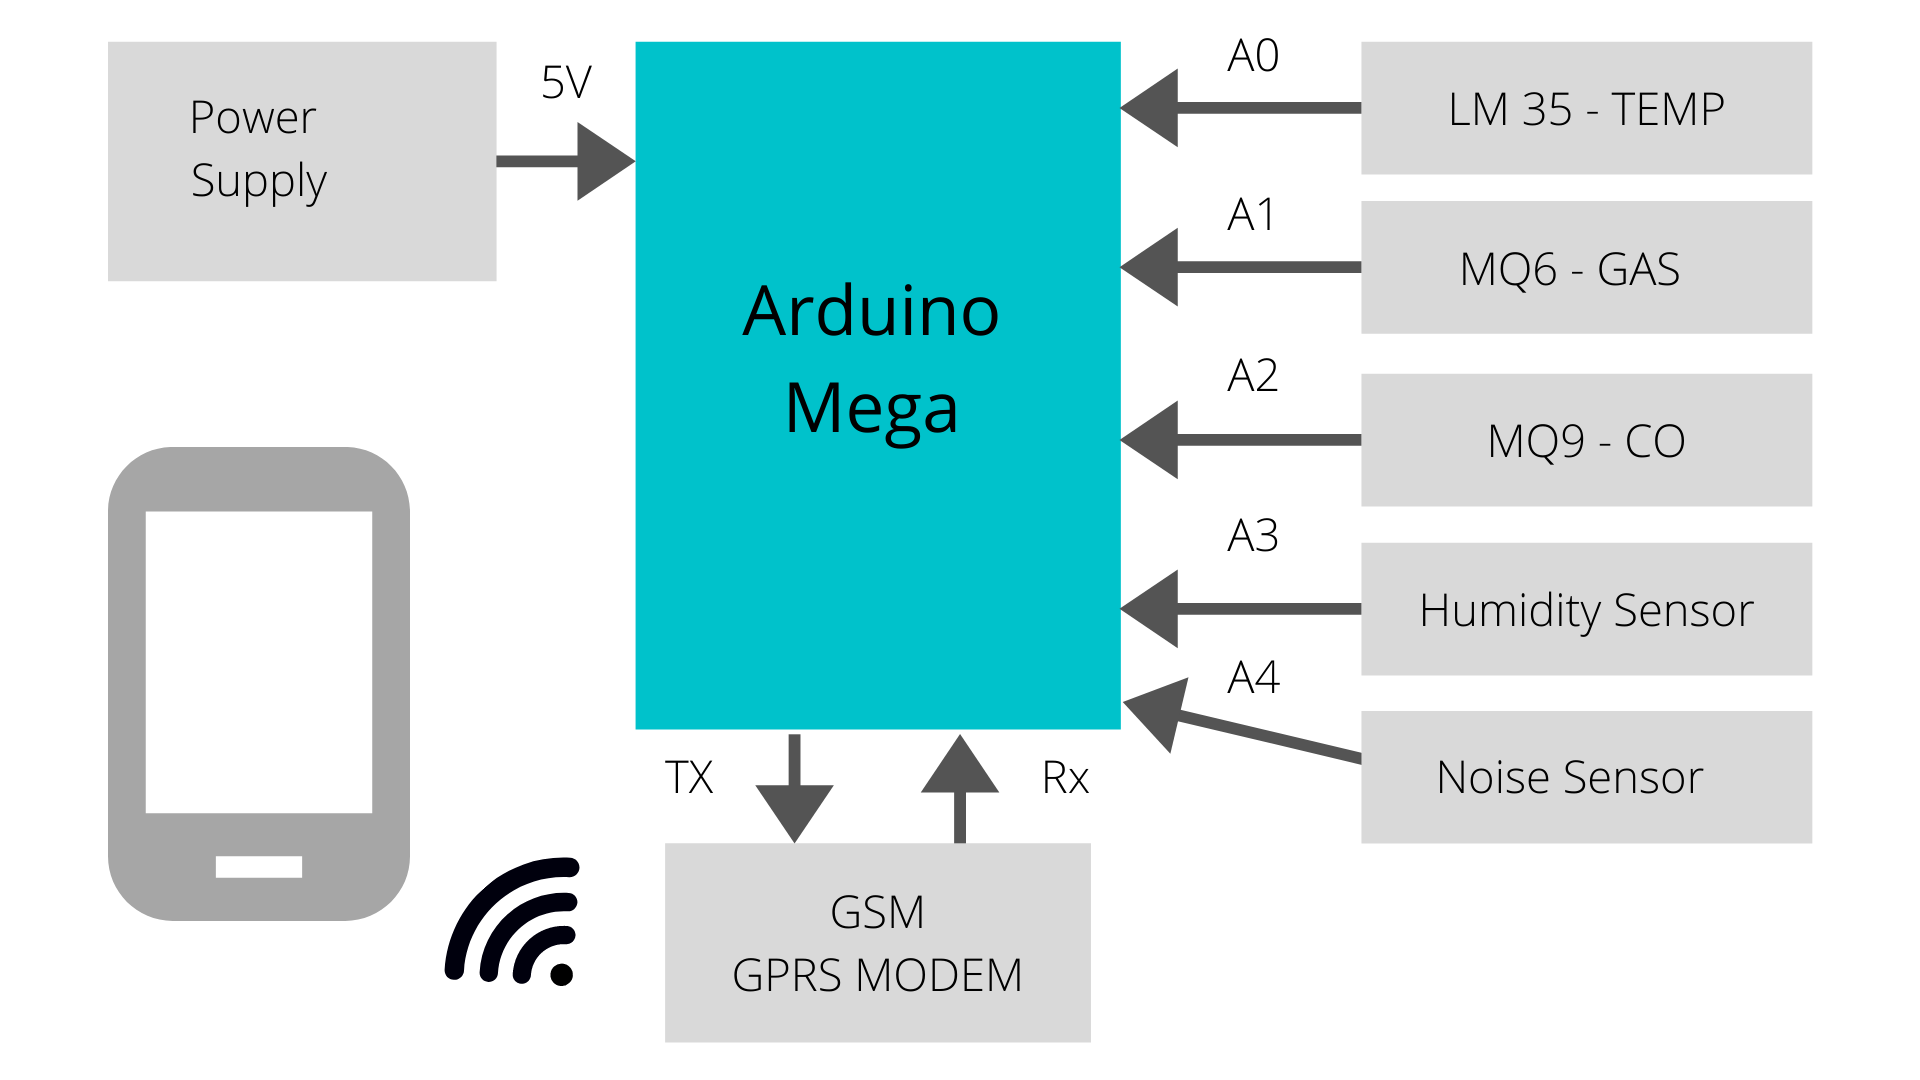
\includegraphics[width=17cm]{title/LM 35 -TEMP.png}
 \caption[]{Schematic Diagram of IoT Based System}
    \label{}
\end{figure}
We have used temperature sensor, gas sensor, $CO$ sensor, humidity sensor and noise sensor.\cite{WinNT} These sensors measures the surrounding conditions and sends the data to the micro-controller. Then the micro-controller sends the data to my device through GSM-GPRS modem. And there is a power supply to the system which is of 5 volt. By this way I can get the information about my surroundings from this system. 
\chapter{Sensors and Equipment}
I have 5 sensors, 1GSM-GPRS modem, 1 arduino mega and power supply. All the equipment are shown in below table:\newline
\begin{table}[h!]
\begin{center}
\begin{tabular}{|c|c|c|}
  \hline
  No. & Equipment Name & Model \\
  \hline
  1 & Temperature Sensor & LM35  \\
  \hline
  2 & Gas Sensor & MQ6  \\
  \hline
  3 & Carbon Monoxide Sensor & MQ9  \\
  \hline
  4 & Humidity Sensor & DHT11  \\
  \hline
  5 & Noise Sensor & KY-038  \\
  \hline
  6 & GPS GSM GPRS Module & SIM900  \\
  \hline
\end{tabular}{}
\end{center}
\caption{Sensors and other equipments}
\label{table:}
\end{table}
\section{Temperature Sensor}
It is an electronic device that measures the temperature of it's environment and converts the input data into electronic data to record, monitor, or signal temperature changes. Here, I have used LM35 sensor. LM35 can Measure the temperature of a particular environment, provide thermal shutdown for a circuit/component, monitor battery temperature, measuring temperatures for HVAC applications. It has 3 pin. One pin is for 4-20 volt input, another is out pin and another is for ground. \cite{liu2011application}
\begin{figure} [h!]
\centering
 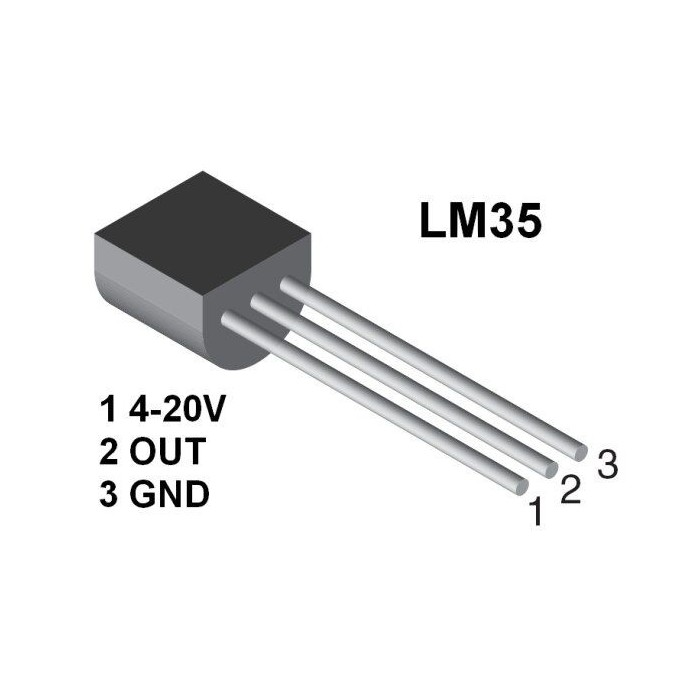
\includegraphics[width=10cm]{Results/lm35.jpg}
 \caption[]{LM35 Temperature Sensor}
    \label{}
\end{figure}
\section{Gas Sensor}
It is an electronic device that is used to detect toxic or explosive gasses and measure gas concentration.. Here, I have used MQ6 sensor. The MQ6 can be used in gas leakage detecting equipment in consumer and industry applications,this sensor is suitable for detecting LPG, iso-butane, propane, LNG. It is consists of a sensing element which comprises of the following parts \cite{evalina2020use}.
\begin{enumerate}[i]
    \item Gas sensing layer
    \item Heater Coil
    \item Electrode line
    \item Tubular ceramic
    \item Electrode
\end{enumerate}
\begin{figure} [h!]
\centering
 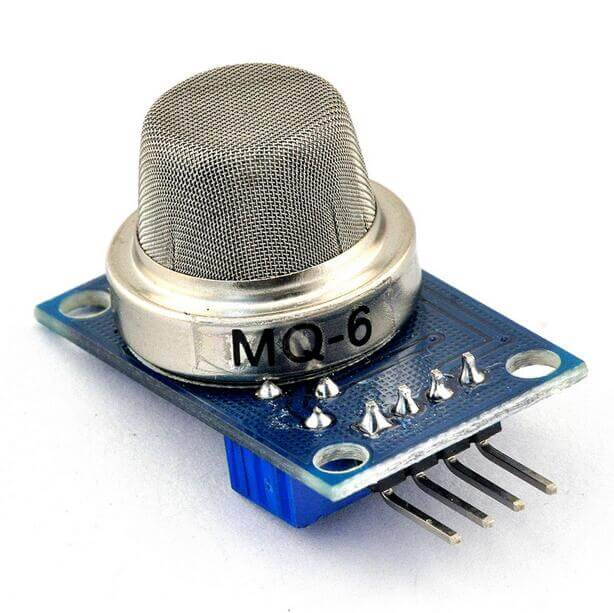
\includegraphics[width=7cm]{Results/MQ6.jpg}
 \caption[]{MQ6 Gas Sensor}
    \label{}
\end{figure}
\section{Carbon Monoxide Sensor}
I have used MQ9 sensor as $CO$ sensor. The MQ-9 Analog Gas Sensor has high sensitivity to Carbon Monoxide, Methane and LPG.\cite{setiawan2018iot}
\begin{figure} [h!]
\centering
 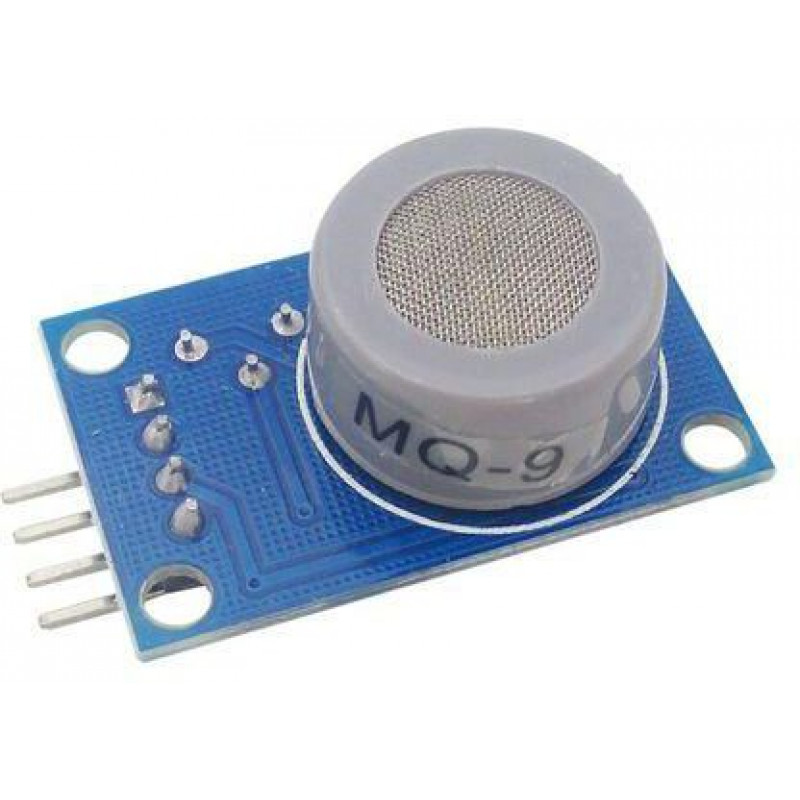
\includegraphics[width=7cm]{Results/mq9.jpg}
 \caption[]{MQ9 $CO$ Sensor}
    \label{}
\end{figure}
\section{Humidity Sensor}
A humidity sensor is an electronic device that measures the humidity in its environment and converts its findings into a corresponding electrical signal. I have used HDT11 as hunidity sensor. It senses, measures and reports both moisture and air temperature. Humidity sensors work by detecting changes that alter electrical currents or temperature in the air.\cite{kuang2007high}
\begin{figure} [h!]
\centering
 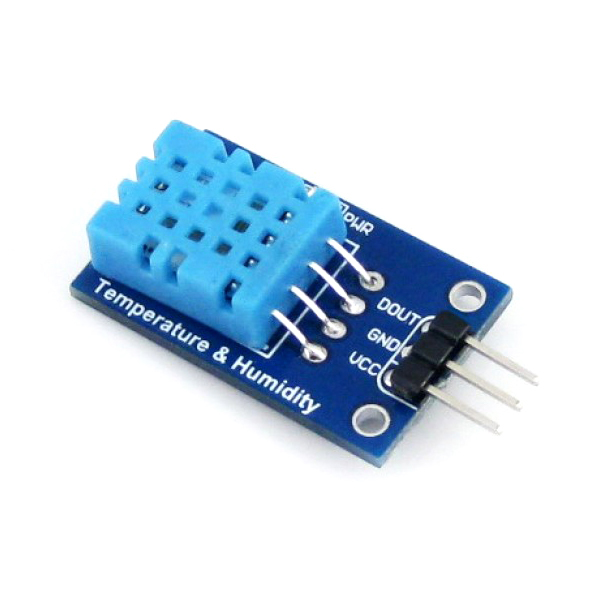
\includegraphics[width=7cm]{Results/hdt111.jpg}
 \caption[]{HDT11 Humidity Sensor}
    \label{}
\end{figure}
\section{Noise Sensor}
I have used KY038 sensor as noise sensor. It sensor is a very basic sound level detector module which features an electric condenser microphone. It is part of a sensor kit that can be purchased and the main part of the module is an LM393 cooperator. \cite{chen2008determining}
\begin{figure} [h!]
\centering
 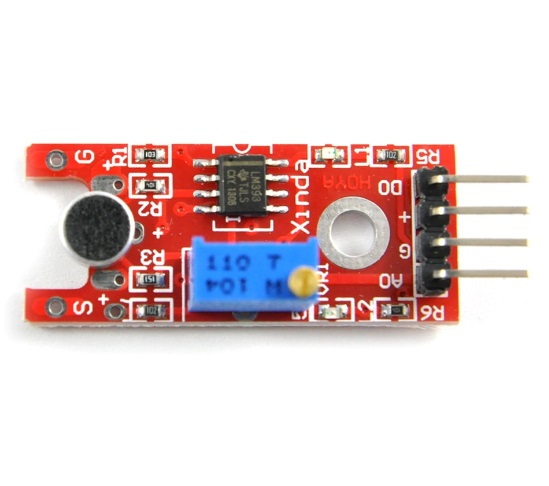
\includegraphics[width=7cm]{Results/ky038.jpg}
 \caption[]{KY038 Noise and Sound Sensor}
    \label{}
\end{figure}
\section{Arduino}
I have used Arduino Mega as micro-controller. The Arduino Mega 2560 is a micro-controller board based on the ATmega2560. It has 54 digital input/output pins (of which 15 can be used as PWM outputs), 16 analog inputs, 4 UARTs (hardware serial ports), a 16 MHz crystal oscillator, a USB connection, a power jack, an ICSP header, and a reset button.\cite{barrett2013arduino}
\begin{figure} [h!]
\centering
 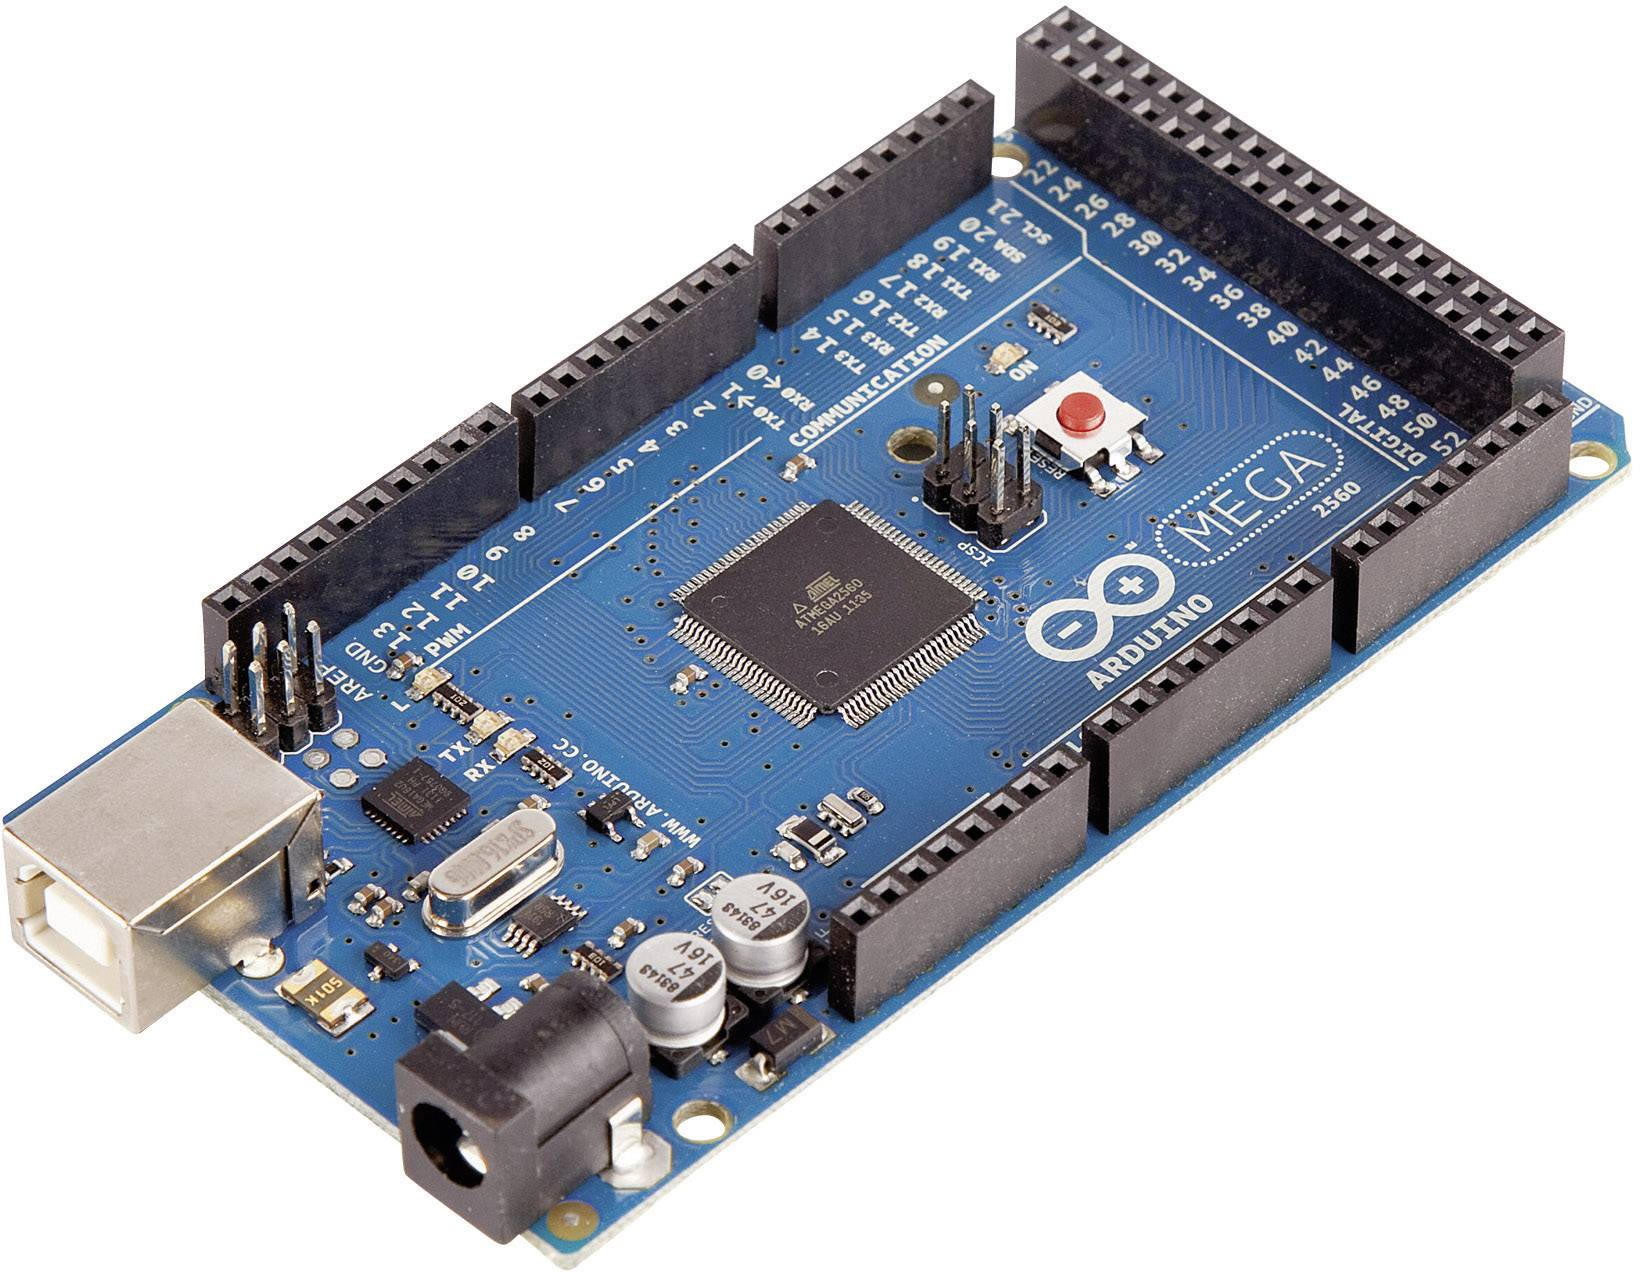
\includegraphics[width=6cm]{Results/arduino.jpg}
 \caption[]{Arduino Mega}
    \label{}
\end{figure}
\section{GPS GSM GPRS Module}
The SIM900 is a complete Quad-band GSM/GPRS solution in a SMT module which can be embedded in the customer applications. ... With a tiny configuration of 24mm x 24mm x 3 mm, SIM900 can fit almost all the space requirements in your M2M application, especially for slim and compact demand of design.\cite{leekongxuesmart}
\begin{figure} [h!]
\centering
 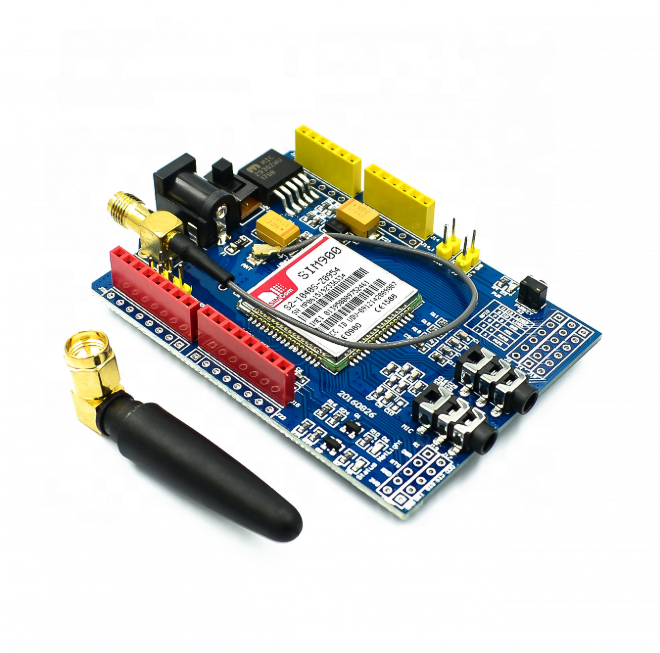
\includegraphics[width=5cm]{Results/900.png}
 \caption[]{GPS GSM GPRS Module}
    \label{}
\end{figure}
\chapter{Solution and Outcome}
LM35, MQ6, MQ9, HDT11 and KY038 will be connected to the arduino board in A0, A1, A2, A3, A4 pin. The SIM900 will be connected to the tx-rx of arduino board. And there will be power supply of 5 volt. Then all the sensors will read the values and send them to the arduino board. It will process them as per the given instruction and then send the prepared result to me using the SIM900. I will be able to know all the information from my mobile.\newline
By this way, I will be able to know-
\begin{enumerate}[1.]
    \item the temperature of my surroundings.
    \item the humidity of my room and outsides.
    \item if there is access sound outside there and I will be able to protect my ears.
    \item if there is any gas leakage.
    \item the amount of Carbon Monoxide of the air.
\end{enumerate}
\bibliographystyle{ieeetr}
\bibliography{bibs/references}
\end{document}